\documentclass{article}
\usepackage[english]{babel}
\usepackage[letterpaper,top=2cm,bottom=2cm,left=3cm,right=3cm,marginparwidth=1.75cm]{geometry}
\usepackage{amsmath}
\usepackage{amssymb}
\usepackage{graphicx}
\usepackage[colorlinks=true, allcolors=blue]{hyperref}
\usepackage{polski}
\usepackage{enumitem}
\usepackage{float}

\title{Metody optymalizacji L3}
\author{Gabriel Budziński\\254609}

\begin{document}
\maketitle

\section{Zadanie 1}

\subsection*{Treść}

W zadaniu należało zaimplementować w języku \texttt{julia} z użyciem pakietu \texttt{JuMP} algorytm 2-aproksymacyjny oparty na programowaniu liniowym dla problemu szeregowania zadań na niezależnych maszynach z kryterium minimalizacji długości uszeregowania.

\subsection*{Algorytm}

Zgodnie z poleceniem kierowano się opisem algorytmu z książki~\cite{vazirani}:
$n$ - liczba zadań, $m$ - liczba maszyn, $LP(T)$ - podproblem szeregowania, w którym czasy wykonania $>$ T nie są brane pod uwagę oraz przyporządkowanie do maszyn jest niebinarne (ciągłe).

\begin{itemize}
    \item obliczenie $\alpha$ - zachłannego ograniczenia górnego,
    \item znalezienie przy pomocy wyszukiwania binarnego najmniejszej wartości $T*$ z przedziału $[\frac{\alpha}{m}, \alpha]$, dla którego $LP(T)$ ma rozwiązanie,
    \item znalezienie korelacji zadań niebinarnie przyporządkowanych do maszyn w wyznaczonym rozwiązaniu
\end{itemize}

\subsection*{Porównanie}

Taki algorytm z założenia powinien być 2-aproksymacyjny, co możemy pokazać, porównując zwrócone przez niego wyniki z wynikami optymalnymi:

\begin{figure}[H]
    \centering
    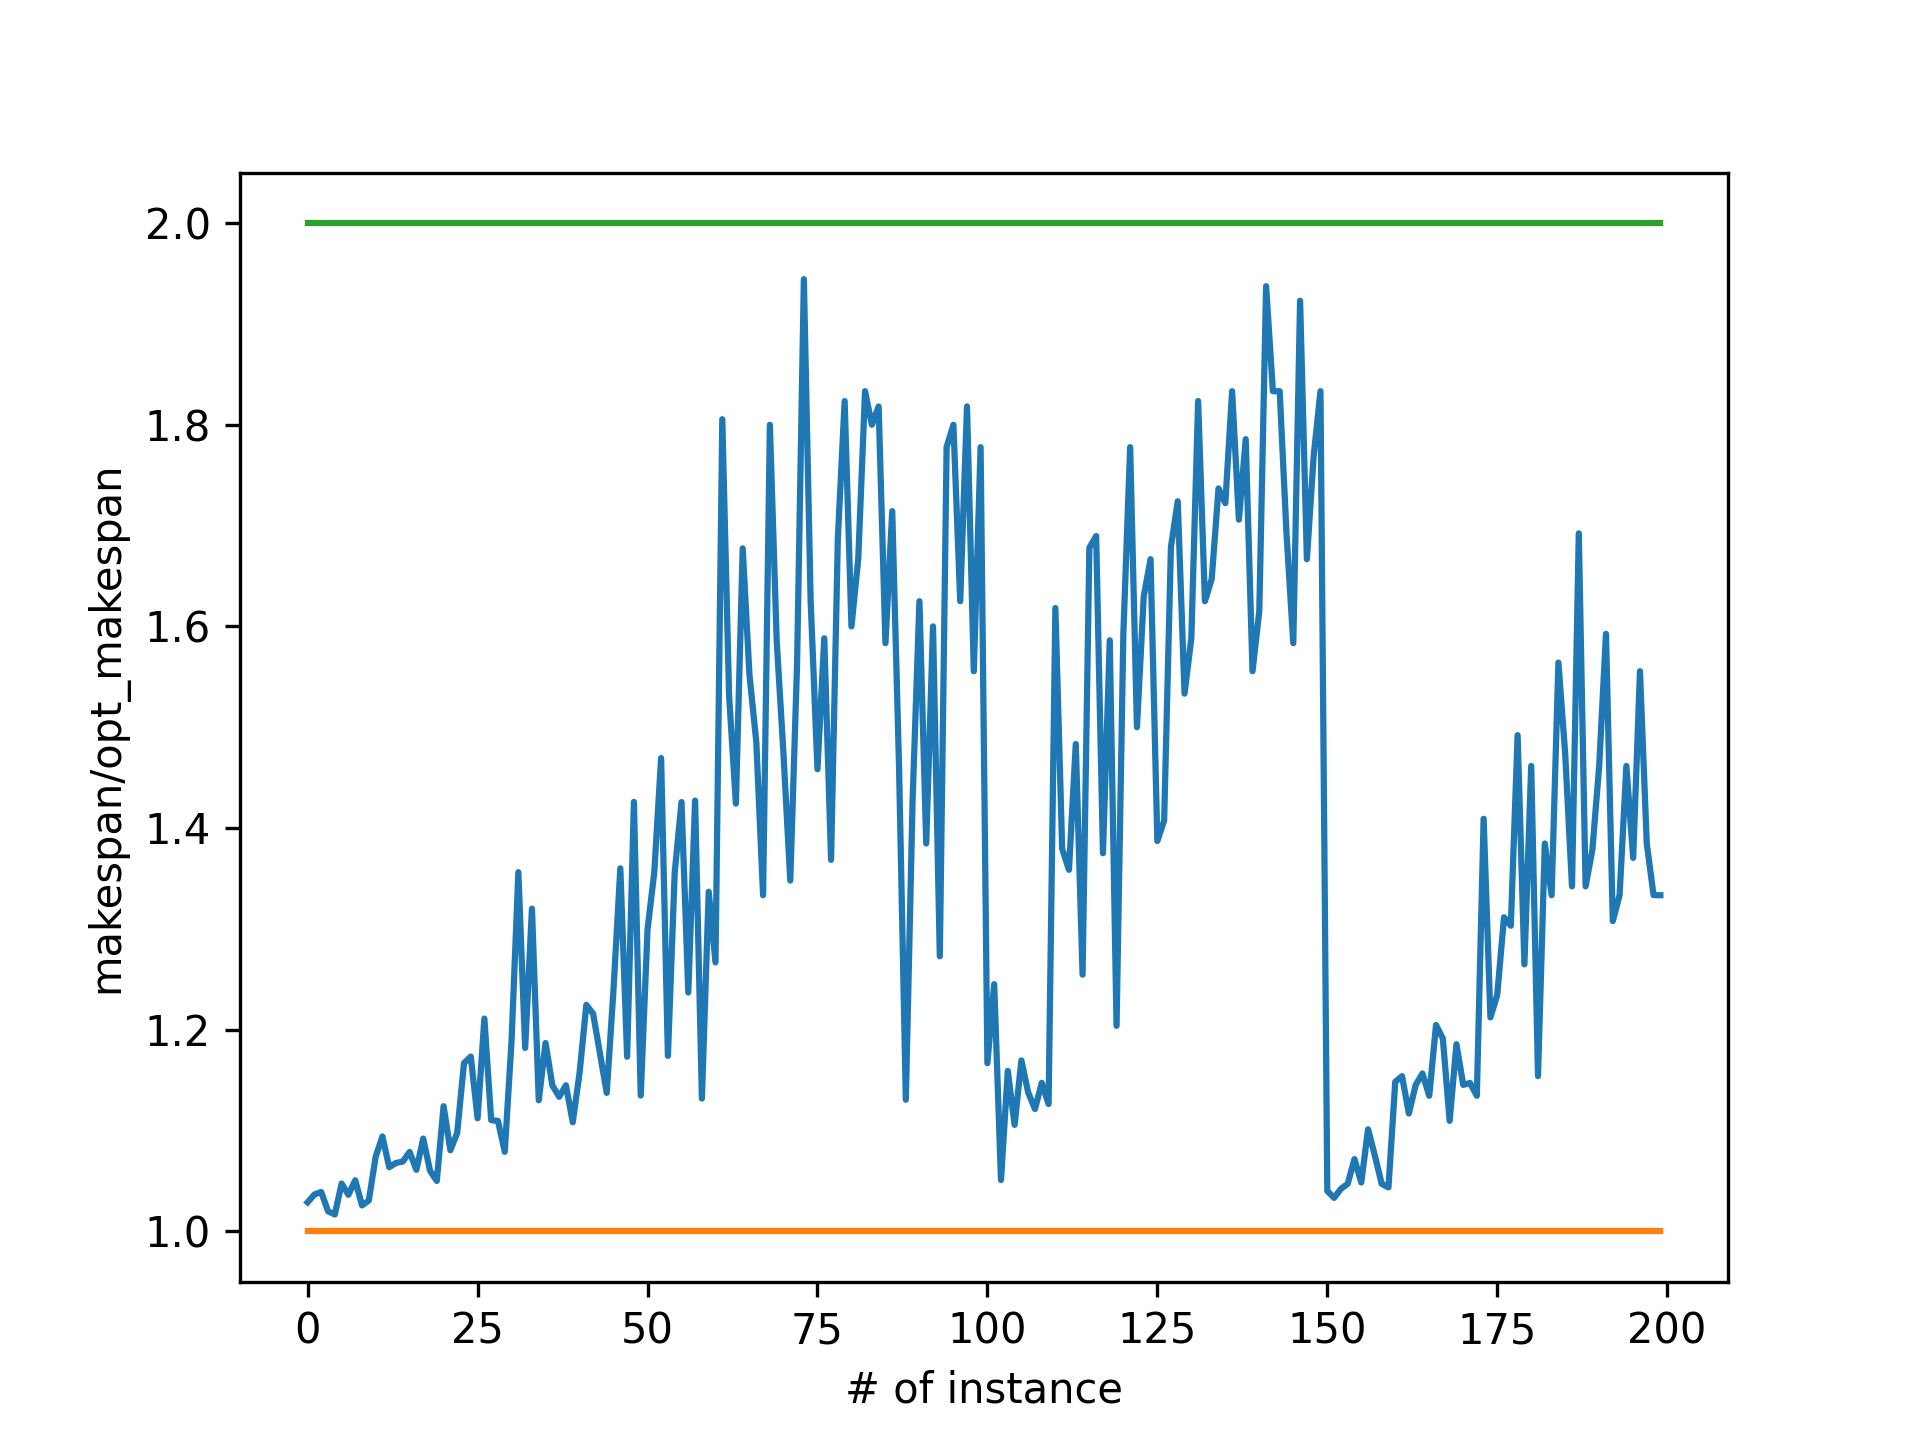
\includegraphics[scale=0.75]{quotients.png}
\end{figure}

Jak widać, alborytm zawsze zwraca wynik będący postaci $c * OPT$, gdzie $c \in [1,2]$

Czas wykonania zaproponowanego algorytmu jest również zadowalający w porównaniu z użytym w bibliotece z instancjami, ze względu na dwie własności - małą wariancję oraz wartość.

\begin{figure}[H]
    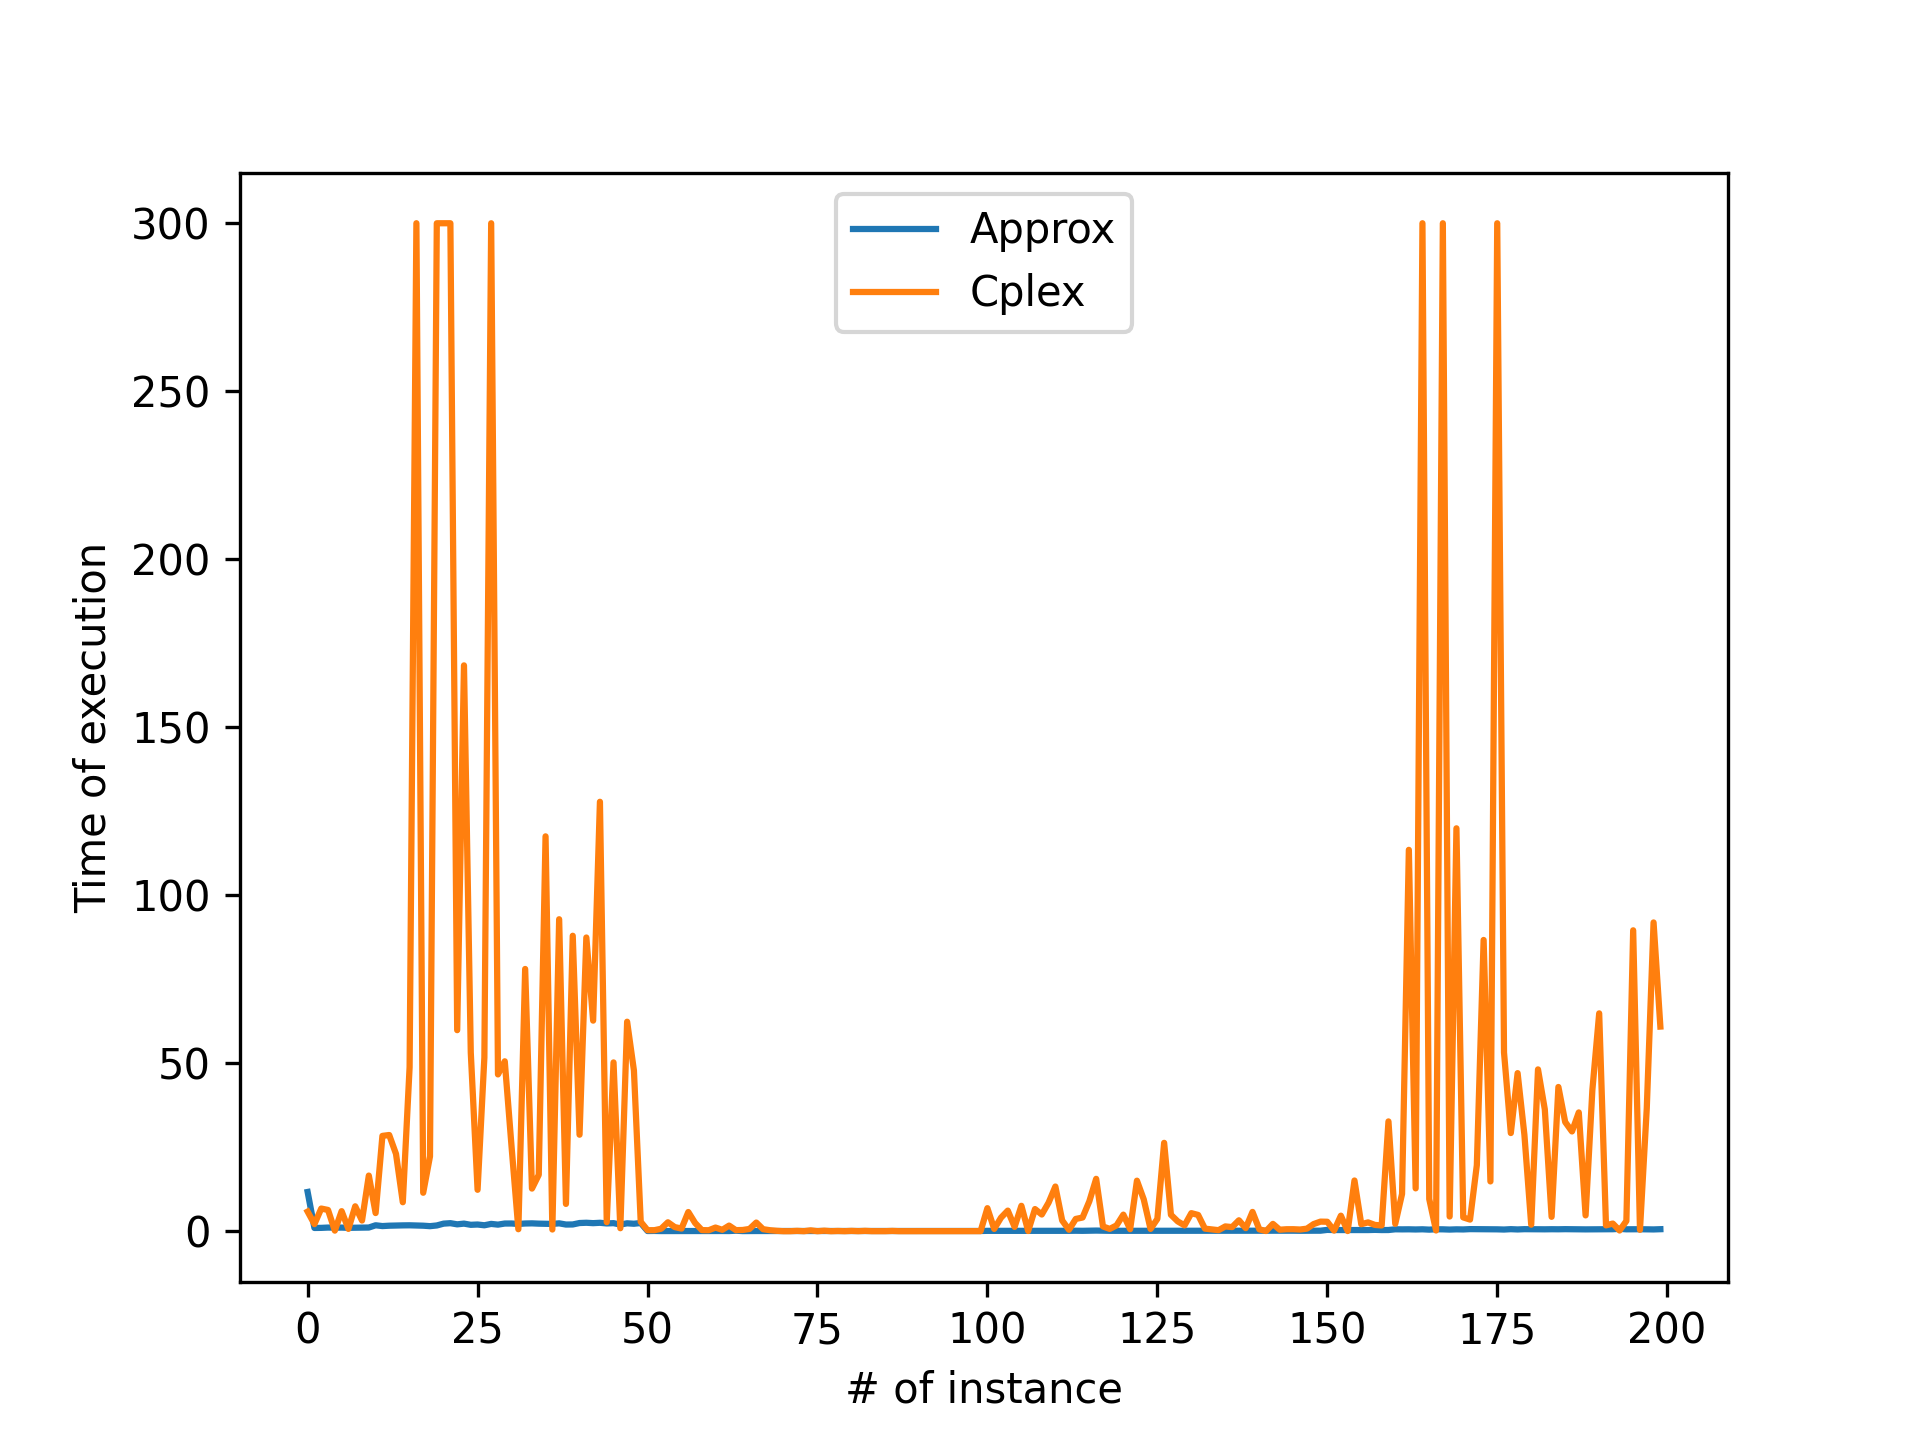
\includegraphics[scale=0.5]{times.png}
    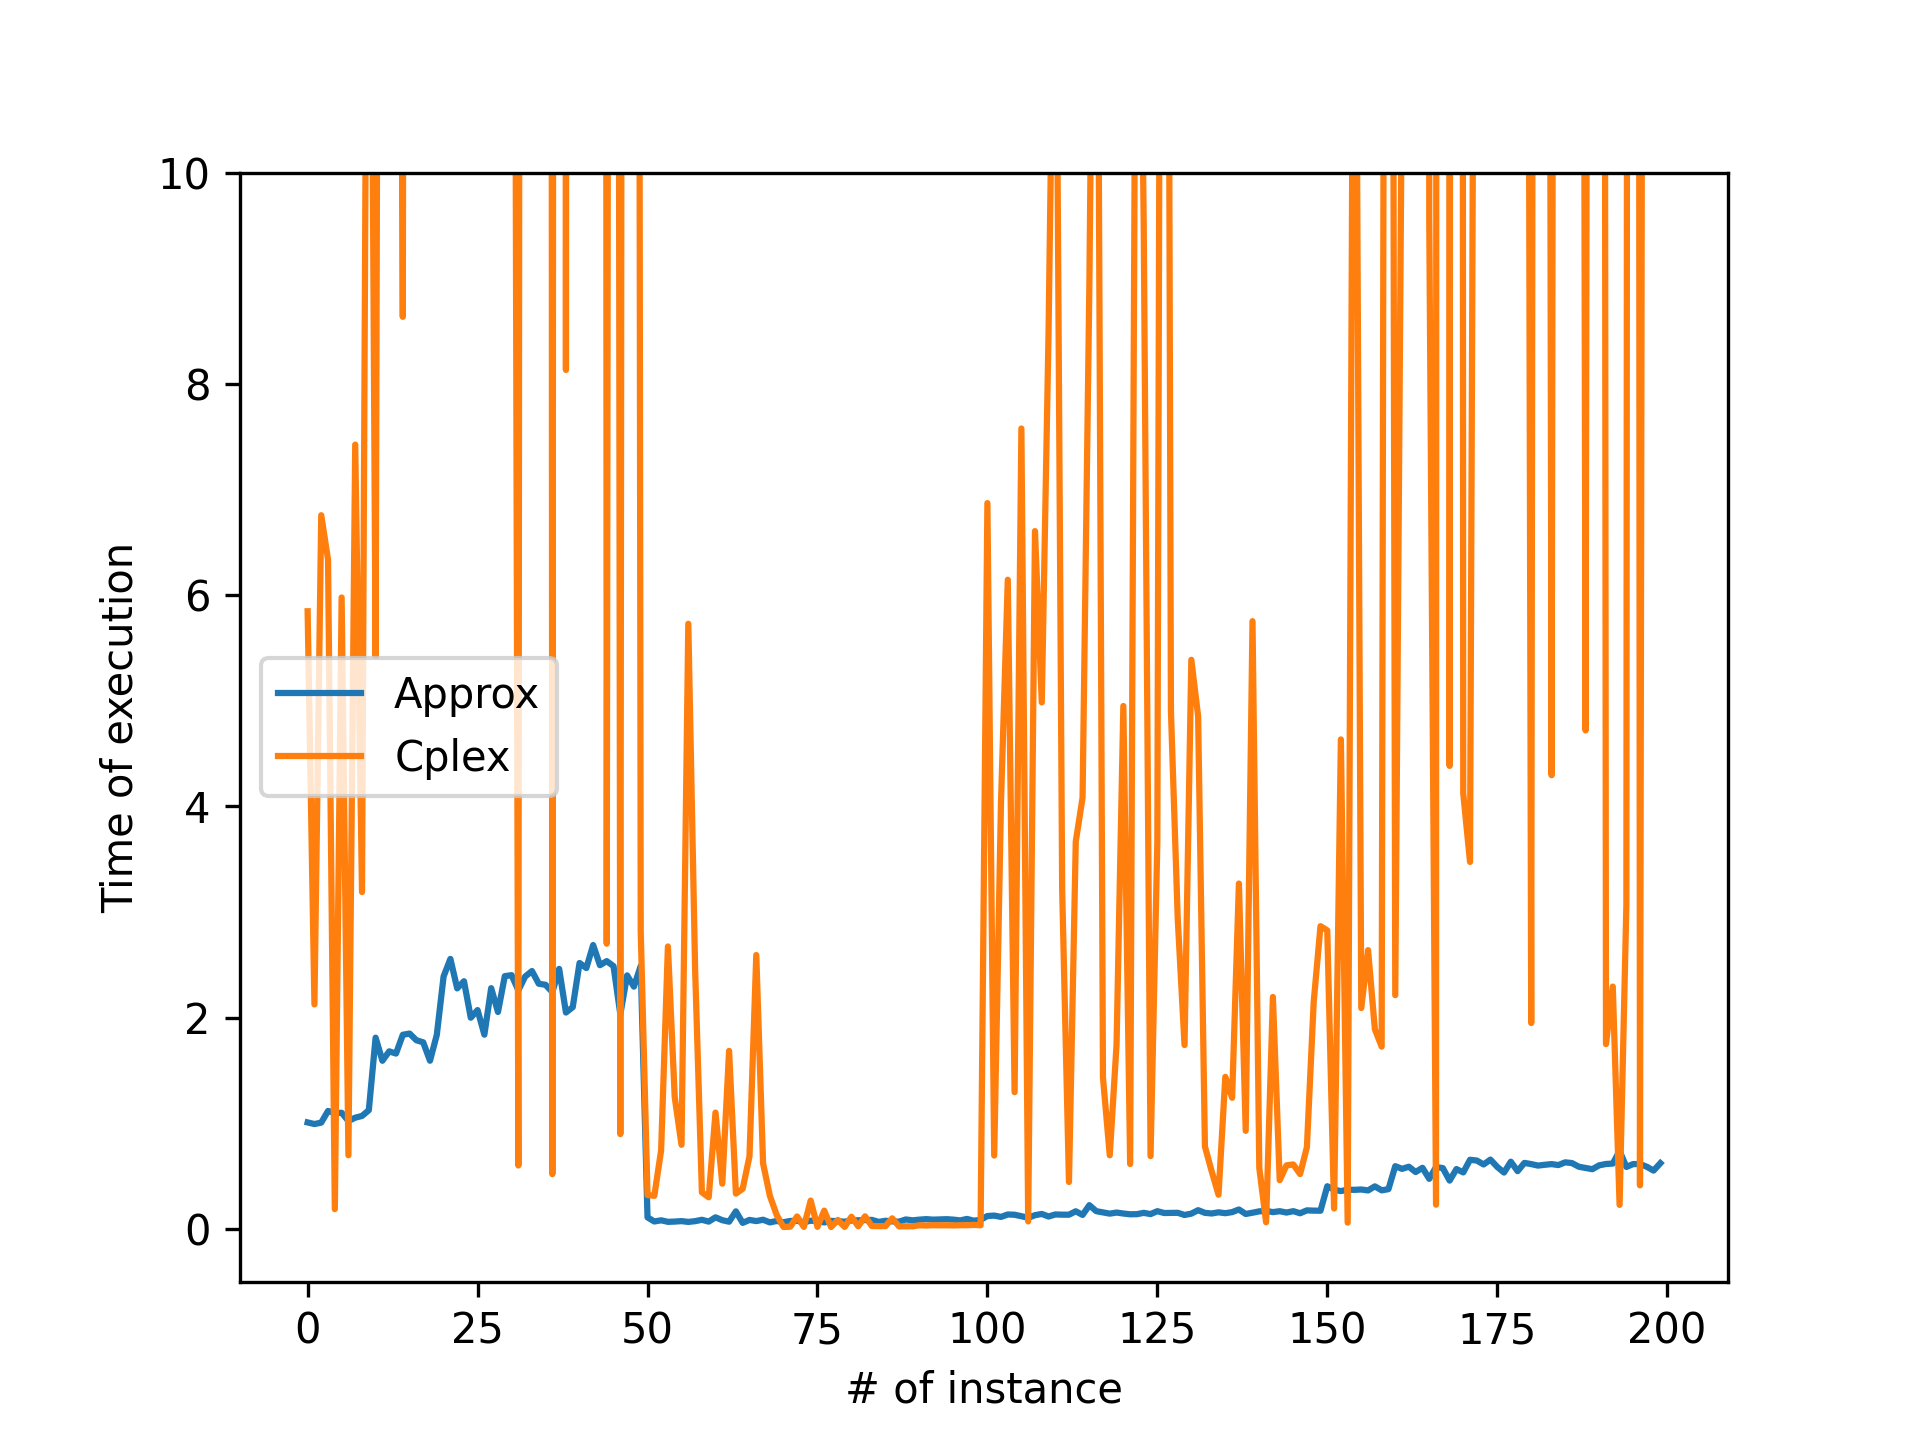
\includegraphics[scale=0.5]{times_lim.png}
\end{figure}


\bibliography{bibliography}
\bibliographystyle{ieeetr}

\end{document}